\documentclass[accentcolor=tud9d,12pt,paper=a4,article]{tudexercise}
\usepackage[utf8]{inputenc}

\title{CV II - Assignment 2}
\subtitle{Dennis Penzel - 1906242 \\ Group 40}
\author{Dennis Penzel (1906242)}
\date{14.06.2017}
\newcommand{\bigCI}{\mathrel{\text{{$\perp\mkern-10mu\perp$}}}}
\begin{document}

\maketitle

\section*{Problem 1}
    \paragraph{1.1}
        A graphical model can display complex structures or problems in a compact, visual way. They are a very efficient way to handle complex problems.
        
    \paragraph{1.2}
        \begin{figure}[h]
        	\centering
        	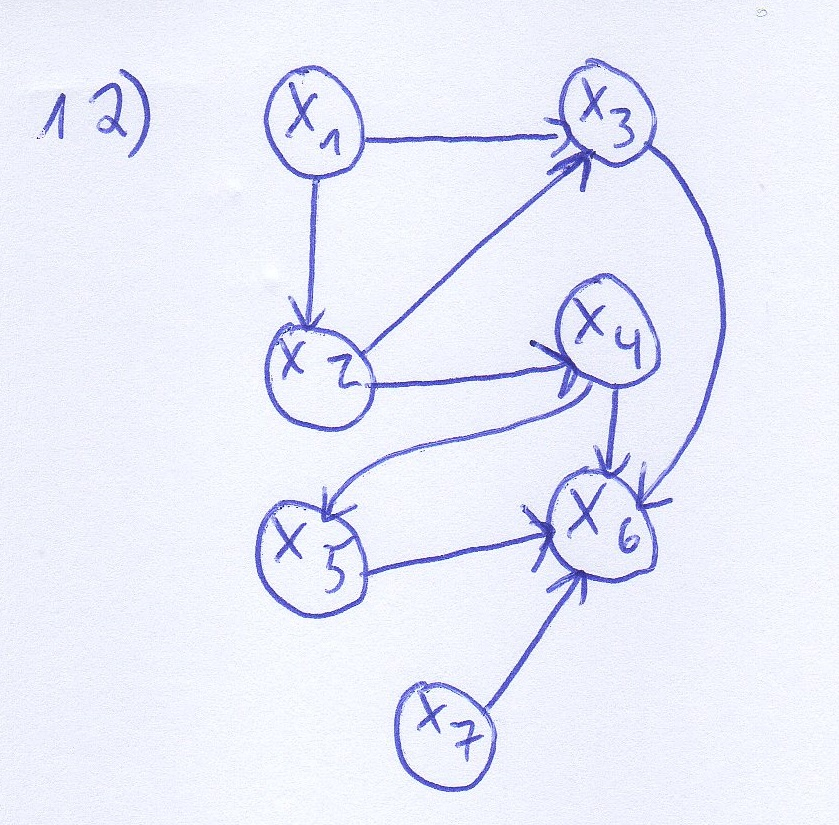
\includegraphics[width=0.4\linewidth]{Figures/a1_2}
        \end{figure}
        Markov blanket of $x_3:\{x_1,x_2\}$
    
    \paragraph{1.3}
    \subparagraph{a)}
        $p(x_1|x_3,x_4,x_5)\ p(x_2)\ p(x_3|x_7)\ p(x_4|x_7,x_8)\ p(x_5|x_4,x_8)\ p(x_6|x_5,x_9)\ p(x_7|x_8)\ p(x_8)\ p(x_9)$
    \subparagraph{b)}
        $\frac{1}{Z}\phi_1(x_1,x_4,x_5)\ \phi_2(x_1,x_3)\ \phi_3(x_4,x_5,x_7,x_8)\ \phi_4(x_3,x_7)\ \phi_5(x_5,x_6)\ \phi_6(x_6,x_9)\ \phi_7(x_2)$
    
    \paragraph{1.4}
        \begin{figure}[h]
        	\centering
        	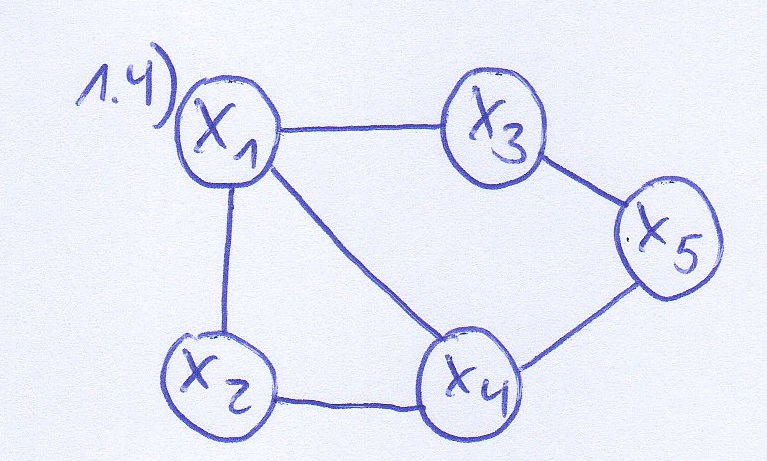
\includegraphics[width=0.3\linewidth]{Figures/a1_4}
        \end{figure}
        \newpage
        
    \paragraph{1.5}
        \begin{table}[h]
            \centering
            \begin{tabular}{c c c|c|c|c|c}
                $x_1$&$x_2$&$x_3$&$\phi_1(x_1)$&$\phi_2(x_2,x_3)$&$\Pi\phi(\dots)$&$p(x_1,x_2,x_3)$ \\\hline
                0 & 0 & 0 & 0,5 & 0+0+1=1 & 0,5 & 0,024 \\
                0 & 0 & 1 & 0,5 & 0+3+1=4 & 2 & 0,095 \\
                0 & 1 & 0 & 0,5 & 2+0+1=3 & 1,5 & 0,071\\
                0 & 1 & 1 & 0,5 & 2+3+1=6 & 3 & 0,143\\
                1 & 0 & 0 & 1 & 0+0+1=1 & 1 & 0,048\\
                1 & 0 & 1 & 1 & 0+3+1=4 & 4 & 0,190\\
                1 & 1 & 0 & 1 & 2+0+1=3 & 3 & 0,143\\
                1 & 1 & 1 & 1 & 2+3+1=6 & 6 & 0,286
            \end{tabular}
        \end{table}
        $\Rightarrow Z=21$
        
    \paragraph{1.6}
    \subparagraph{a)}
        Fig.2 left:\\ $x_2 \bot x_1 | x_3$\\
        $\Rightarrow x_3$ blocks all routes from $x_2$ to $x_1$
        
    \subparagraph{b)}
        Fig.2 right:\\ $x_2 \bot x_1$\\
        $\rightarrow$ Markov blanket of $x_2=\{x_3\}$\\ $\Rightarrow$ independent of $x_1$
    
    \paragraph{1.7}
        \subparagraph{1.}
	        \begin{figure}[h]
	        	\centering
	        	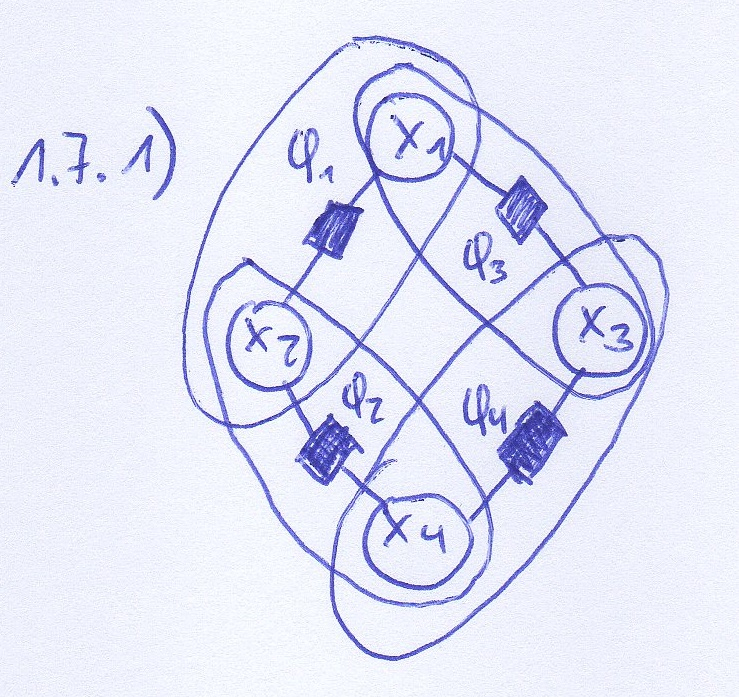
\includegraphics[width=0.3\linewidth]{Figures/a1_7_1}
	        \end{figure}
            $\frac{1}{Z}\phi_1(x_1,x_2)\ \phi_2(x_2,x_4)\ \phi_3(x_1,x_3)\ \phi_4(x_3,x_4)$
        \subparagraph{2.}
	        \begin{figure}[h]
	        	\centering
	        	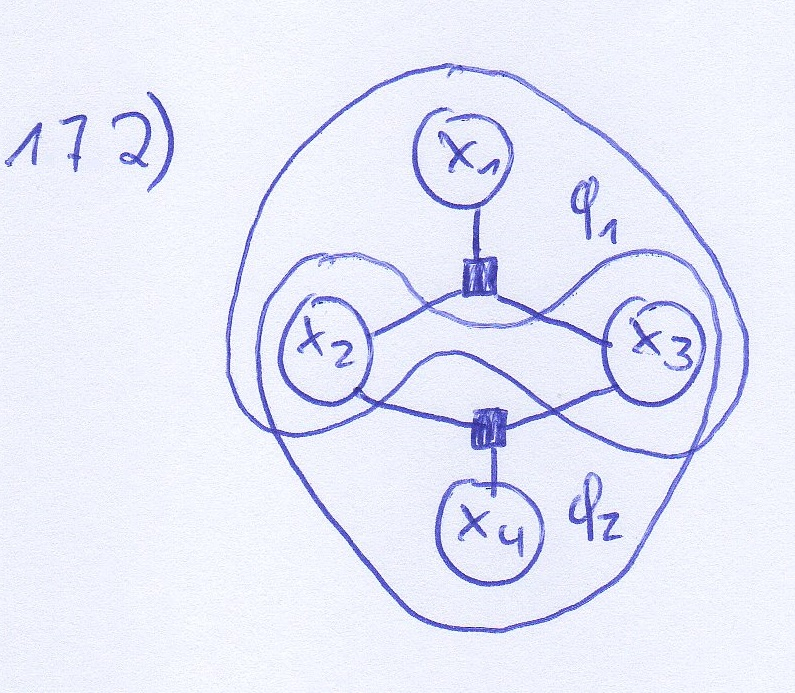
\includegraphics[width=0.3\linewidth]{Figures/a1_7_2}
	        \end{figure}
            $\frac{1}{Z}\phi_1(x_1,x_2,x_3)\ \phi_2(x_2,x_3,x_4)$
        \subparagraph{3.}
	        \begin{figure}[h]
	        	\centering
	        	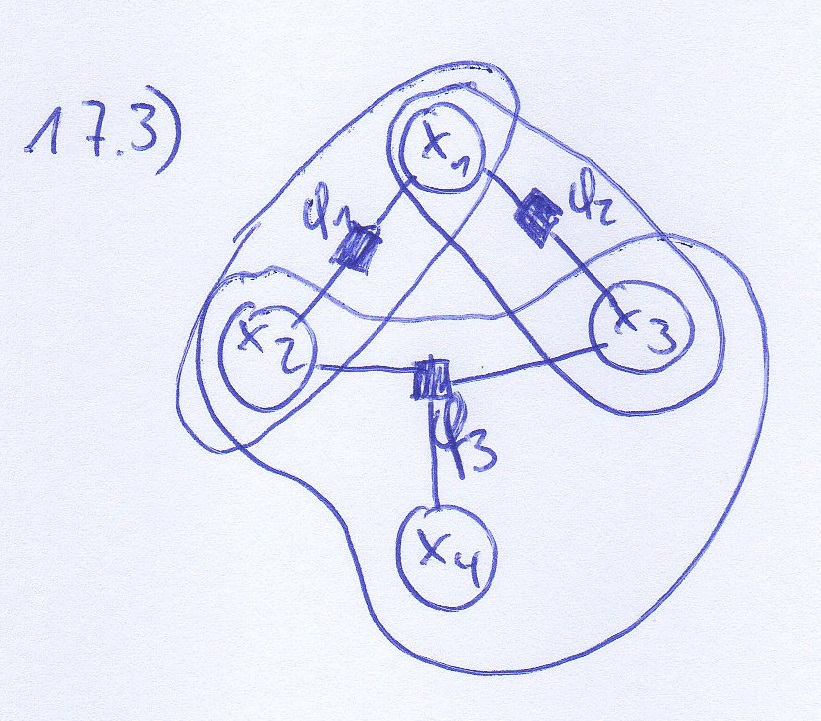
\includegraphics[width=0.3\linewidth]{Figures/a1_7_3}
	        \end{figure}
            $\frac{1}{Z}\phi_1(x_1,x_2)\ \phi_2(x_1,x_3)\ \phi_3(x_2,x_3,x_4)$
            
    \paragraph{1.8}
        $\{w_2,w_4,w_6,w_6,x_5\}$
    \paragraph{1.9}
        $\{w_2,w_3,w_5,x_4\}$
        
\section*{Problem2}
    \paragraph{2.1}
        $
        p(L=0|S=0)\\ \\
        =\frac{p(L=1,S=0)}{p(S=0)} = \frac{\sum_R p(L=1,S=0,R)}{\sum_{R,L} p(S=0,R,L)}
        =\frac{p(L=1,S=0,R=0)+p(L=1,S=0,R=1)}{p(L=1,S=0,R=0)+p(L=1,S=0,R=1)+p(L=0,S=0,R=0)+p(L=0,S=0,R=1)}\\ \\
        =\frac{0,7\cdot0,7\cdot0,1+0,9\cdot0,3\cdot0,1}{0,7\cdot0,7\cdot0,1+0,9\cdot0,3\cdot0,1+0,3\cdot0,7\cdot0,9+0,8\cdot0,3\cdot0,9} = \frac{0,049+0,027}{0,049+0,027+0,189+0,216}=\frac{0,076}{0,481}\\ \\
        \underline{\underline{\approx 0,158}}
        $
    \paragraph{2.2}
        $
        p(L=1|S=0,R=0)\\ \\
        =\frac{p(L=1,S=0,R=1)}{\sum_L p(L,S=0,R=1)} = \frac{p(L=1,S=0,R=1)}{p(L=1,S=0,R=1)+p(L=0,S=0,R=1)}\\ \\
        =\frac{p(S=0|R=1,L=1)\cdot p(R=1)\cdot p(L=1)}{p(S=0|R=1,L=1)\cdot p(R=1)\cdot p(L=1)+p(S=0|R=1,L=0)\cdot p(R=1) \cdot p(L=0)}\\ \\
        =\frac{0,9\cdot0,3\cdot0,1}{0,9\cdot0,3\cdot0,1+0,8\cdot0,3\cdot0,9}=\frac{0,027}{0,027+0,216}=\frac{0,027}{0,243}\\ \\
        \underline{\underline{= 0,\overline{1}}}
        $
    \paragraph{2.3}
        The observation that there are no free seats left creates an dependency between the two events L and R. Now, with the addition that we observe the raid outside, the probability that L=1 decreases. This event (R=1) provides an additional explanation for our S=0 and intuitively lowers our believing that L=1. So we can say that the observation of R=1 'explains away' the observation of S=0.
\end{document}
